% !TeX root = responsiveness_tr
%% ================================================================
\section{Problem}\label{prresp_Problem}

Common implementations of DCTCP~\cite{Alizadeh10:DCTCP} (e.g.\ in Linux or FreeBSD) take two rounds before a change in congestion on the path fully feeds into the moving average that regulates its response. This is on top of the inherent round trip of delay that the feedback loop adds.

Both extra rounds are due to the two-stage process for maintaining the EWMA then using it to respond to congestion. The first stage introduces a round of delay while it accumulates the marking fraction before passing the EWMA to the second stage that uses it to respond to congestion. The second extra round of delay is because the first stage clocks independently, while the second stage is triggered by the onset of congestion. So it takes two rounds before a full round of the congestion that triggered the start of the second stage has fed through into the EWMA that the first stage passes to the second.

\section{Per-ACK EWMA}\label{prresp_Per-Packet_EWMA}

Instead of the EWMA of the marking probability being upscaled by a constant factor, it is proposed to upscale it by \texttt{flight\_ / gain} (where \texttt{flight\_} is the packets in flight, and \texttt{gain < 1} is a constant). Then, as shown below, the EWMA can be maintained by a single continuous set of repetitive increments or decrements determined on each ACK.

As we shall see, scaling up the EWMA by \texttt{flight\_} enables the repetitive per-packet operations to implicitly smooth the EWMA with a characteristic timescale proportionate to the RTT (specifically, \texttt{RTT/gain}).

This contrasts with the two-stage process of accumulating the marking fraction for a round before feeding it into an EWMA that is explicitly clocked per round.

The scaled up EWMA is effectively a smoothed count of the number of congestion marks per RTT (\texttt{v = p*flight\_}), but scaled up by the constant \texttt{1/gain}. 

Common implementations of DCTCP incorrectly mimic the timing but not the size of a classic congestion control's response. Classical congestion controls suppress any further response for a round because their initial response is large. On first onset of congestion, it seems wrong for DCTCP to immediately respond with a tiny reduction (based on the previous absence of congestion), then suppress any further response for a round trip. 

Once we have an EWMA of congestion marks that is updated continually on every ACK, it becomes possible to spread the reduction over the round. Then, during the round, \texttt{v} will be growing if congestion is rising, and the response will naturally grow accordingly.

\paragraph{Definitions of variables}
\begin{description}[nosep]
	\item [\texttt{g}] = \texttt{1/gain}. By default \texttt{g = 16};
	\item [\texttt{g\_shift}] = \texttt{lg(g)};
	\item [\texttt{av\_up}]: EWMA of the marks per round upscaled by \texttt{g}; Alternatively, it might help to think of this as the EWMA of the marking probability (alpha in DCTCP) upscaled by \texttt{g * flight\_}. 
	\item [\texttt{flight\_}]: the number of packets in flight when the marking probablity was fed into the EWMA;
	\item [\texttt{flight}]: the number of packets in flight now;
	\item [\texttt{ce\_fb}] = 1 ECN packet feedback; 0 otherwise.
\end{description}

\subsection{Intuition}\label{prresp_intuition}

In DCTCP, the EWMA, \texttt{alpha}, is maintained per round trip as follows (in floating point arithmetic):
\begin{verbatim}
    alpha += (F - alpha)/g,
\end{verbatim}
where F is the fraction of marked bytes accumulated over the last round trip.

This can be approximated (see \S\,\ref{prresp_approx}) by repeatedly updating the EWMA on the feedback of every packet, but scaling down each update by the number of packets in that round, \texttt{flight\_}. That is, the following per-packet update:
\begin{verbatim}
    alpha += (ce_fb - alpha) / (flight_*g).
\end{verbatim}

The above per-packet update of the EWMA is roughly equivalent to the following per-packet update of the upscaled EWMA, \texttt{av\_up}:
\begin{verbatim}
    av_up += ce_fb - av_up/(flight_*g).
\end{verbatim}

\subsection{Implementation}\label{prresp_implementation}

\subsubsection{Maintaining the EWMA}

The \texttt{ce\_fb} term can be implemented by adding 1 to \texttt{av\_up} on feedback of each CE-marked packet. If the upscaling of \texttt{av\_up} by \texttt{g} were removed to produce an EWMA of marks per round, this would be equivalent to adding \texttt{1/g} of a mark.

The number of packets acknowledged in the current round is \texttt{flight}. So repeatedly subtracting \texttt{av\_up/(flight\_*g)} on the arrival of every ACK would reduce \texttt{av\_up} by \texttt{av\_up*flight/(flight\_*g)} in a round. This approximates to \texttt{av\_up/g} per round. In integer arithmetic, that can be implemented by \texttt{av\_up/g} decrements of 1. 

This is achieved as shown %in \autoref{fig:prresp_per-ack-ewma_av_up} 
below by the repetitive additions, comparisons and decrements of a variable called \texttt{av\_carry}, which carries forward the remainder between ACKs. 

We have defined the general-purpose function \texttt{repetitive\_div()} for the repetitive division, which will be reused later for maintaining the congestion window as well.

%\begin{figure*}
\begin{verbatim}
On_each_ACK'd_packet {
    av_up += ce_fb - repetitive_div(
              av_up, flight*g, &av_carry);
}

/* Repeated execution outputs true with 
 *  frequency proportional to numerator 
 *  (num) divided by denominator (denom)
 */
bool repetitive_div(u32 num, u32 denom, 
                            u32 *carry) {
    *carry += num;
    if (*carry > denom) {
        *carry -= denom;
        return true;
    }
    return false;
}
\end{verbatim}
%\caption{Per-ACK maintenance of an EWMA of marks per round}
%\label{fig:prresp_per-ack-ewma_av_up}
%\end{figure*}

\autoref{fig:per-ack-ewma-verify} compares toy simulations of the above EWMA and the DCTCP EWMA (without changing cwnd). It can be seen that, when whenever marks arrive, the algorithm always moves immediately, whereas DCTCP's EWMA does nothing until the next round trip cycle.
\begin{figure}
	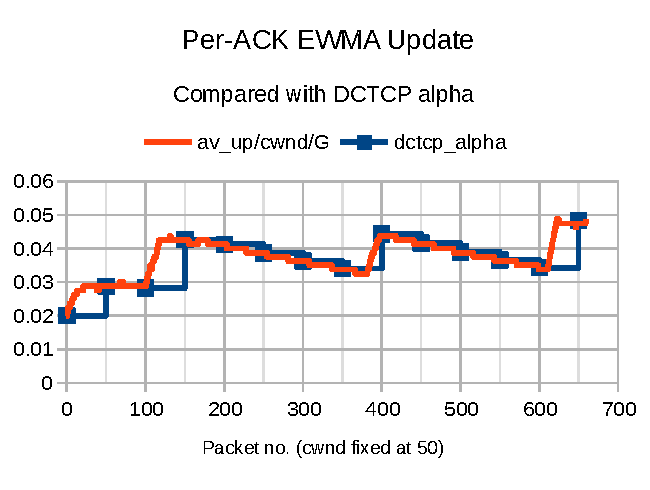
\includegraphics[width=\linewidth]{per-ack-ewma-verify}
	\caption{Initial verification of per-ACK EWMA algorithm, with constant \texttt{cwnd}}\label{fig:per-ack-ewma-verify}
\end{figure}

\subsubsection{Responding to Congestion}\label{prresp_congestion_response}

The proposed approach uses the teaching of DCTCP selectively. DCTCP reduces \texttt{cwnd} by \texttt{alpha*cwnd/2} in any round trip in which CE feedback is present. The proposed approach reduces \texttt{cwnd} by half the average number of marked packets per round, or \texttt{av\_up / (2*g)}. 

This is broadly equivalent to DCTCP in that it maintains the scalable '\(1/p\)' response function, but with two main quantitative differences:
\begin{itemize}[nosep]
	\item The window reduction is taken as a proportion of what the window has been in recent rounds, not what it is now (as in DCTCP) (see \S\,\ref{prresp_Non-Concerns}).
	\item The window reduction is taken as a proportion of the amount of the window that has been \emph{used} in recent rounds, not the maximum that the flow was entitled to use, i.e.\ packets in flight not \texttt{cwnd}. Thus, if an application-limited flow has only used a quarter of the available window in recent rounds, the proposed reduction of \texttt{cwnd} will be only a quarter of that applied by DCTCP.
\end{itemize}

The main departure from DCTCP is in the speed of response. Rather than reduce  \texttt{cwnd} on the first sign of CE feedback then suppress further response for a round trip, it is proposed to spread the reduction over the round following the first sign of CE feedback. In other words, use the whole round while in CWR state to reduce \texttt{cwnd} as the EWMA updates, such that, by the end of the round it will still have reduced as much as it would have done if the whole reduction had been applied at the end of CWR state.

This will exploit the fact that the EWMA (\texttt{av\_up}) is continually updated on every ACK. So, at one extreme, if the first CE mark is immediately followed by many others, the EWMA will rapidly increase early in the round of CWR, and \texttt{cwnd} can be rapidly decreased accordingly. While, at the other extreme, if the first CE mark is the only CE mark in the round, \texttt{cwnd} will still have reduced by \texttt{alpha*cwnd/2} by the end of the round, but the EWMA will hardly have increased above the value it took when the CWR round started.

To spread the reduction over the round, the proposed algorithm below does not divide the round into an arbitrary number of points where \texttt{cwnd} is altered by varying amounts. Instead, it alters \texttt{cwnd} on the first ACK when the algorithm calculates that at least one packet of movement is in order. 


\begin{verbatim}
On_each_ACK'd_packet {
    av_up += ce_fb - repetitive_div(
              av_up, flight*g, &av_carry);
    if (!cwr && ce_fb) {
        // Record start of CWR state
        cwr = true;
        next_seq = snd_next;
    }
    if (cwr) {
        cwnd -= repetitive_div(
          av_up, flight*g*2, &cwnd_carry);
        // Check for end of CWR round
        if (snd_una > next_seq) {
            cwr = false;
        }
    }
}

\end{verbatim}

\bob{Consider inflating cwnd reduction by cwnd/flight.}

\section{(Non-)Concerns}\label{prresp_Non-Concerns}

There seems to be a circular dependency, because \texttt{av\_up} is both upscaled by \texttt{cwnd} then used to update \texttt{cwnd}.

In fact, \texttt{av\_up} is upscaled by what \texttt{cwnd} \emph{was} at the time of each repetitive decrement or increment of \texttt{av\_up}. So  \texttt{av\_up} depends on an implicit exponentially weighted moving average of \texttt{cwnd} with a characteristic smoothing timescale of \texttt{g} round trips. This stabilizes the circular dependency.

\section{Evaluation}\label{prresp_Evaluation}

For research purposes, we ought not to introduce two changes at once, without evaluating each separately. Therefore, initially, we ought to use the continually updated EWMA, \texttt{av\_up} to reduce \texttt{cwnd} in the classical way. That is, on the first feedback of a CE mark, reduce \texttt{cwnd} once by \texttt{av\_up/(2*g)}. Then suppress further response for a round (CWR state). This should remove one round of lag (originally spent accumulating the marking fraction), but not the other (reducing cwnd in response to a single mark, then doing nothing for a round while the extent of marking is becoming apparent).

Basic experiments will need to compare how quickly a DCTCP flow in congestion avoidance can reduce in response to a newly arriving flow. It will also be necessary to check performance in the following more cases that might expose poor approximations in the algorithm (relative to DCTCP):
\begin{enumerate}
	\item When the packets in flight has been growing for some time;
	\item \ldots{}or shrinking for some time;
	\item When the flow is application limited, with packets in flight varying wildly, rather than tracking the smoother evolution of \texttt{cwnd}.
\end{enumerate}

\section{Related Work}\label{prresp_related}

Reducing \texttt{cwnd} by half of \texttt{v} per round trip is similar to Relentless TCP~\cite{Mathis09:Relentless}, which reduces \texttt{cwnd} by half a segment on feedback of each CE-marked packet. The difference is that \texttt{v} is a moving average, so it implements smoothing in the sender, whereas Relentless immediately applies a full congestion response without smoothing, because it is designed for smoothing in the network.

Like DCTCP, the per-ACK congestion response proposed in section 5.2 of \cite{Alizadeh11:DCTCP_Analysis} maintains an EWMA of congestion marking probability, \texttt{alpha}. But it reduces \texttt{cwnd} by half of \texttt{alpha} (in units of packets) on feedback of each ECN mark. This causes jumpiness, because marks tend to be bunched into one round then clear for a few rounds, particularly with step-marking. So, even though this algorithm uses the smoothed EWMA for each reduction, it applies many more reductions in those rounds with more marks. In contrast, the approach proposed in the present paper limits the reduction to \texttt{alpha} within a round trip (as DCTCP itself does). Nonetheless, it removes the round of lag that DCTCP's EWMA uses to accumulate the marking probability, and it spreads the reduction over a round to ensure that it picks up feedback as soon as it arrives.

\section{Future Work}\label{prresp_future}

\bob{Possibility of increasing gain (reducing g).}
\bob{Possibility of adding reduction proportional to growth in av\_up (adding the P part of a PI controller).}
\bob{Possibility of using av\_up to detect that the flow probably gone open-loop, and should enter a different mode to find a faster operating point. E.g.\ measuring the number of unmarked packets since the last mark, and using the difference between that and the average distance implied by av\_up.}
